\subsection{Why does bureaucracy exist? Can't we just do the work?}

how does bureaucracy come into existence?
* complexity of problem


https://en.wikipedia.org/wiki/Libertarianism

The minimal scenario to start from is to imagine a single person working on a single task that does not last long (a few minutes), is relatively easy (cognitively and physically and emotionally), and does not recur. Most of what you do occurs outside those limits and thus incurs some concept of \gls{process} (breaking a task into subtasks). Staying with the one-person constraint, a complex task can benefit from being broken into subtasks where order of the subtasks matters. 




% https://graphthinking.blogspot.com/2021/09/why-is-everything-so-hard-in-large.html

What if we completely avoided bureaucracy? Try replacing ``bureaucracy" in that question with ``coordination of stakeholders". If you avoid coordination of stakeholders, what you get is random interactions. 

What if we minimized bureaucracy? Again, try replacing ``bureaucracy" in that question with ``coordination of stakeholders". The goal of ``minimizing coordination" probably isn't the real objective. To be more precise, a specific objective might be ``minimize time spent executing the task" (which takes a lot of coordination prior to the task execution) or ``minimize the level of distraction to stakeholders" (chunk the coordination time). Another strategy for minimizing bureaucracy is to reduce the number of stakeholders involved. For a given task complexity, this means having smarter people who have more skills. 

\begin{figure}
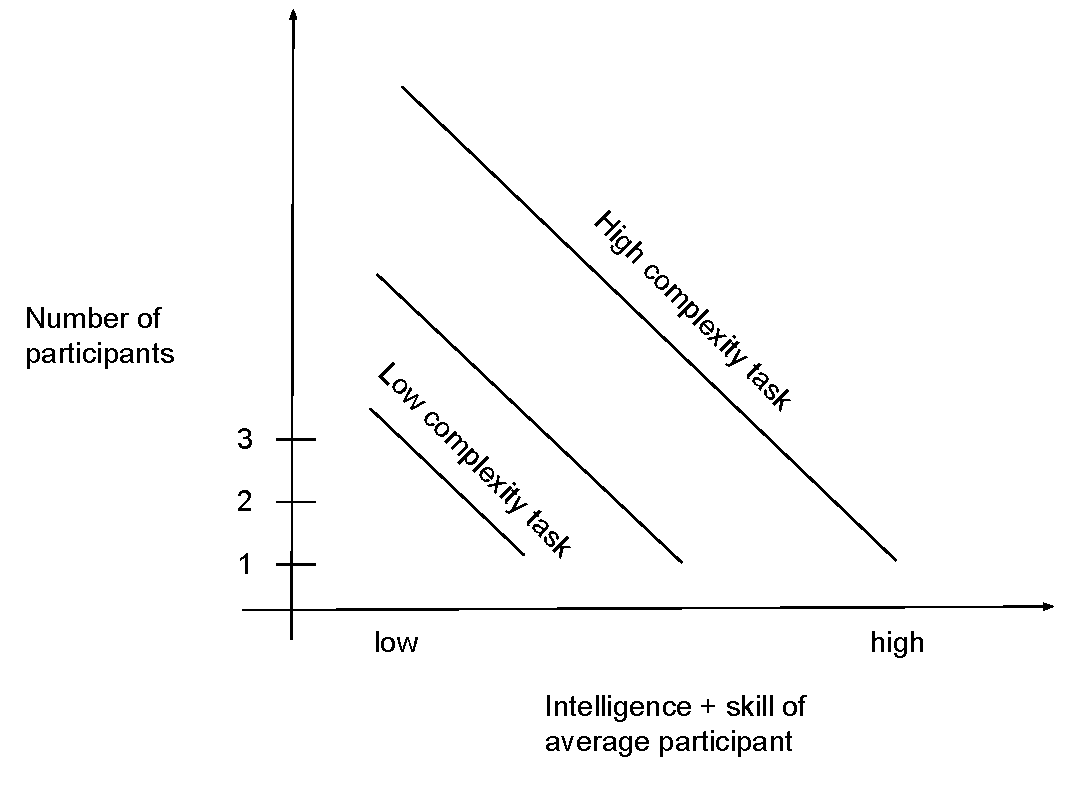
\includegraphics[width=0.8\textwidth]{images/people-per-task-for-skill-level.pdf}
\caption{Three levels of task complexity are shown. As task complexity increases, the size of the team needs to grow. The growth may be less if the team members are brilliant. Those brilliant people cost more and there are fewer of them.}
\end{figure}
